\documentclass{article}
\usepackage{graphicx}  % For including images
\graphicspath{{front_page/}}
\usepackage[a4paper,margin=15mm]{geometry}  % Page size and margins
\usepackage{multicol}  % For two-column layout
\usepackage[finnish]{babel}
\usepackage{fontspec}  % To use custom fonts
\usepackage{titlesec} % For customizing section titles
\usepackage{xcolor}    % For changing text color
\usepackage[colorlinks=true, linkcolor=cyan, urlcolor=cyan]{hyperref}
\setmainfont{Bai Jamjuree}  % Set Bai Jamjuree as the main font
\pagenumbering{gobble}

\usepackage{fancyhdr} % For customizing the header and footer
\pagestyle{fancy} % Enable fancy page style
\renewcommand{\headrulewidth}{0pt} % Remove header line
\fancyfoot[C]{Luotu \today} % Custom text in the center of the footer

% Define colors (example for Pinkki)
\usepackage{xcolor}
\definecolor{bg1}{HTML}{FFB2E3}
\definecolor{bg2}{HTML}{FFD9F2}
\definecolor{hl}{HTML}{FF00A2}
\definecolor{border}{HTML}{660044}

% Adjust paragraph settings
\setlength{\parindent}{0pt} % Disable paragraph indentation
\setlength{\parskip}{2em} % Add vertical space between paragraphs

\titlespacing*{\subsection}
  {2em}                        % Increase indentation of subsection title
  {0.5em}                      % Reduce vertical space before the subsection
  {0.5em}                      % Reduce vertical space after the subsection
\titlespacing*{\section}
  {0em}                        % Increase indentation of subsection title
  {2em}                      % Reduce vertical space before the subsection
  {0em}                      % Reduce vertical space after the subsection
\setlength{\parindent}{0em} % paragraph indentation
\setlength{\parskip}{.7em} % vertical space between paragraphs

% Hyphenation control parameters
\hyphenpenalty=100000 % Higher values reduce the likelihood of hyphenation
\exhyphenpenalty=1000 % Discourages hyphenating compound words
\lefthyphenmin=3 % Minimum number of characters at the beginning of a hyphenated word
\righthyphenmin=3 % Minimum number of characters at the end of a hyphenated word
\tolerance=10000 % Controls line-breaking tolerance (lower values discourage hyphenation)
\pretolerance=100 % Line-breaking tolerance before attempting hyphenation

\begin{document}
	%\\\vspace{0.5em} % Adjust the space between the title and subtitle
    %\Large{hyppynarun tasojärjestelmä yksilönarulle} % Subtitle in a slightly smaller font

\noindent\begin{minipage}[t]{0.22\textwidth} % Left column (narrower)
	\vspace*{-3em}
	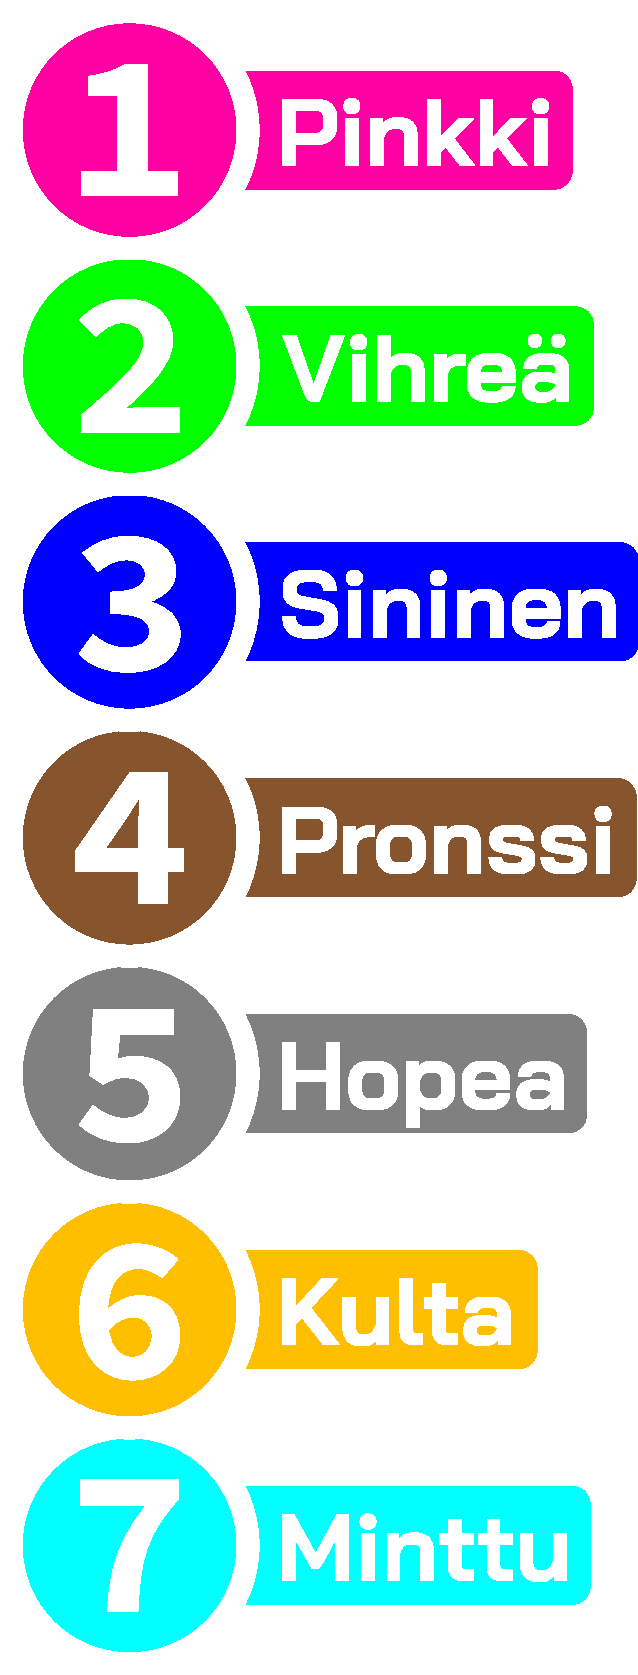
\includegraphics[width=\textwidth]{titles.pdf}  % Replace with your actual file
\end{minipage}%
\hfill% Add space between the two minipages
\begin{minipage}[t]{0.75\textwidth} % Right column (wider)
    {\Huge \bfseries Sinkkunarun tasojärjestelmä} % Main title in large font

	\setlength{\parindent}{0em} % paragraph indentation
	\setlength{\parskip}{.7em} % vertical space between paragraphs
	\vspace*{5mm}
	Sinkkunarun tasojärjestelmä on monipuolinen kokoelma
	hyppynaruliikkeitä ja \mbox{-liikesarjoja}, jotka on jaettu seitsemään eri tasoon
	helpoimmasta (taso 1) vaikeimpaan (taso 7). Jokaisella tasolla on oma
	kaksisivuinen \emph{tasopassi}, johon liikkeet ja sarjat voi merkitä
	opituiksi. Kun koko tasopassi on suoritettu, hyppijä pääsee etenemään
	seuraavalle tasolle. Mikään ei kuitenkaan estä harjoittelemasta myöhempien
	tasojen liikkeitä jo aikaisemmin.

	Tasojärjestelmä sisältää monipuolisesti sinkkunarukilpailuissa tarvittavia
	liikkeitä: vuoroaskel (speed step), kaksois- ja komoishypyt, sekä kaikki
	pakolliset freestyle-temppukategoriat (käsirajoitteet, heitot ja wrapit,
	akrobatia, monikertahypyt). Järjestelmä rajoittuu vain sinkkunaruun, eli se
	ei sisällä Double Dutch ja Wheel \mbox{-yhteistyölajeja}.

	Hyppynaruvalmennuksessa tasojärjestelmää voidaan käyttää pelillistämään
	oppimista ja rohkaisemaan omatoimista harjoittelua palkitsemalla hyppääjää
	jokaisesta suoritetusta tasosta kyseisen tason värisillä hyppynaruhelmillä.
	Helmet voi sitten pujottaa vaikka kengän nauhaan merkiksi saavutetuista
	taidoista.

	Koska liikkeiden ja liikesarjojen opettelu paperilta voi olla hankalaa,
	jokaisen tason liikkeet ja sarjat on videoitu. Mallivideot löytyvät
	\href{https://www.youtube.com/@RopeSkippingHelsinki}{Rope Skipping Helsingin
	YouTube-kanavalta} tasokohtaisilta soittolistoilta, joihin pääsee suoraan
	tasopassin alalaidan QR-koodista.
\end{minipage}

\vspace*{-1em}
\section*{Tasopassin käyttöohjeet sivu 1: yksittäiset liikkeet}
Tasopassin ensimmäisellä sivulla on lista suoritettavia liikkeitä. Jokaisella
rivillä on liikkeen nimi ja laatikko, jonka voi rastia, kun liike on suoritettu
annettujen vaatimusten mukaisesti.
\vspace*{-.5em}
\begin{center}
	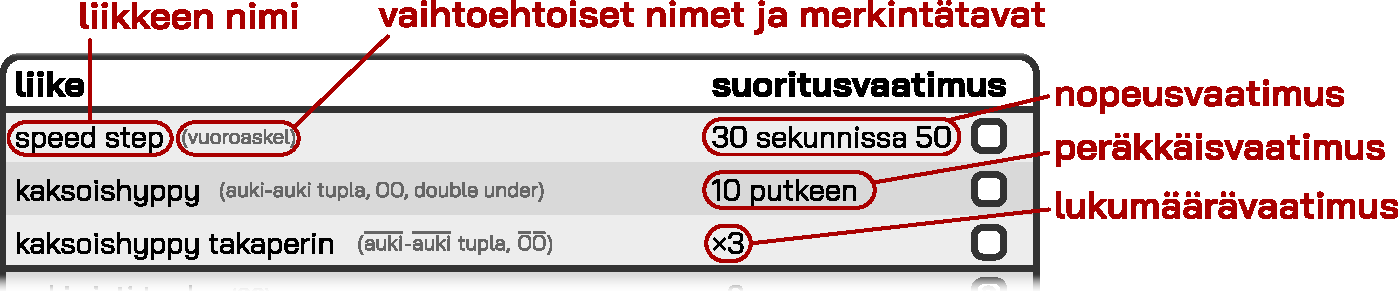
\includegraphics[scale=.75]{skill_table_example.pdf}
\end{center}
\vspace*{-.5em}
Suoritusvaatimuksia on kolmenlaisia. Niistä yleisin, \emph{lukumäärävaatimus},
kertoo kuinka monta peräkkäistä onnistunutta suoritusta tarvitaan. Esimerkiksi
``kaksoishyppy takaperin ×3'' tarkoittaa, että hyppääjän täytyy tehdä 3
takaperin tuplaa ilman epäonnistuneita yrityksiä välissä. Tuplahyppyjen välillä
saa kuitenkin hyppiä perushyppyjä tai pitää taukoa, eli niiden \textbf{ei
tarvitse olla tehty putkeen}. Mutta jos tuplahyppyä yrittäessä tapahtuu virhe,
täytyy laskeminen aloittaa nollasta. Yritys lasketaan onnistuneeksi, kun hyppijä
tekee sekä suoritettavaa liikettä ennen että sen jälkeen vähintään yhden
perushypyn.

\emph{Peräkkäisvaatimus} tarkoittaa, että suoritusten välissä ei saa tehdä
perushyppyjä tai pitää taukoa, vaan liikket on tehtävä putkeen. Jos liike on
useamman hypyn pituinen, peräkkäisvaatimuksessa lasketaan kokonaisia
suorituksia, ei yksittäisiä hyppyjä. Esimerkiksi vuoroaskel on kaksi hyppyä
pitkä (yksi hyppy oikealla ja yksi vasemmalla jalalla), joten peräkkäisvaatimus
``vuoroaskel 4 putkeen'' tarkoittaa yhteensä kahdeksaa (8) hyppyä.

\emph{Nopeusvaatimus} koskee vain vuoroaskelta (speed step) ja tuplia (double
under), joissa kilpaillaan nopeudessa. Näissä virheet eivät haittaa kunhan
riittävä määrä onnistuneita suorituksia tulee täyteen annetussa ajassa.

\begin{minipage}[t]{0.8\textwidth} % Left column (narrower)
	\setlength{\parindent}{0em} % paragraph indentation
	\setlength{\parskip}{.7em} % vertical space between paragraphs
	Tyhjä suoritusmerkintälaatikko
	\raisebox{-0.7ex}{
\includegraphics[scale=.75]{tickbox_empty.pdf}}
	tarkoittaa, että liike on pakollinen tasopassin suorittamiseksi.
	Numeroidut laatikot
	\raisebox{-0.7ex}{
\includegraphics[scale=.75]{tickbox_1.pdf}} ja %
	\raisebox{-0.7ex}{
\includegraphics[scale=.75]{tickbox_2.pdf}}
	sen sijaan eivät ole pakollisia, vaan niitä ruksimalla
	kerätään pisteitä. Vaadittu pistemäärä on ilmoitettu taulukon vieressä
	harmain luvuin. Esimerkiksi
	\raisebox{-0.3ex}{
\includegraphics[scale=.75]{kategoriapisteet.pdf}}
	tarkoittaa, että tämän kategorian osalta tasopassin suorittamiseksi riittää
	kerätä 5 pistettä 8 pisteen maksimipistemäärästä. Kategorioiden rajat on
	merkitty taulukkoon paksuin vaakaviivoin.

	Jos jollain liikkellä on kaksi suoritusmerkintälaatikkoa, on kyseinen liike
	epäsymmetrinen, eli sen voi suorittaa sekä oikealla että vasemmalla
	puolella. Esimerkkejä epäsymmetrisistä liikkeistä ovat erilaiset ristit ja
	käännökset sekä perushyppy yhdellä jalalla.
\end{minipage}%
%\hfill% Add space between the two minipages
\begin{minipage}[t]{0.2\textwidth} % Right column (wider)
	\vspace*{0em}
	\raggedleft%
	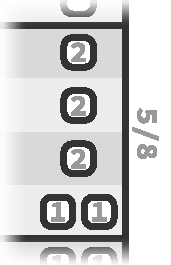
\includegraphics[scale=.75]{kategoriaesimerkki.pdf}
\end{minipage}%
\newpage
\vspace*{\paperheight}

\end{document}
